\subsection{逐图分布：平均值之外的结构异质性}
五点平均曲线是赛题指定的主结果，但均值不能描述一百张图之间的离散程度。为避免只列举最好的例子，表\ref{tab:fivecore-quantiles}从冻结逐例账本取五核逐图加速比的最小值、十分位、四分位、中位数、四分之三位、九十分位和最大值。分位数按排序后作线性插值；它是描述这一百张给定图的经验分布，不是未知总体的概率分位数。问题一的中位数 $4.310373$ 高于均值 $3.665903$，反映一批低加速图把算术平均拉低；问题二的中位数 $4.648439$ 亦高于均值 $4.159974$。这比只说“有些图较难”更具体：算法已有大量接近五倍的配置，但低分位结构仍值得定向检查。
\begin{table}[!htbp]\centering\small
\caption{五核逐图加速比的经验分位数（100图）}\label{tab:fivecore-quantiles}
\begin{tabular}{lrrrrrrr}
\toprule
场景 & 最小 & 10\% & 25\% & 中位数 & 75\% & 90\% & 最大\\
\midrule
问题一：A & 1.001729 & 1.590521 & 2.442082 & 4.310373 & 4.909619 & 4.996015 & 5.501141\\
问题二：B & 1.678167 & 2.539582 & 3.553248 & 4.648439 & 4.921746 & 5.036342 & 5.827795\\
\bottomrule
\end{tabular}
\end{table}

图\ref{fig:fivecore-cdf}从全部一百张图绘制经验累积分布，而不是选取几个“代表图”。纵坐标为 $\widehat F(s)=100^{-1}\sum_i\mathbf1\{S_{i,5}\le s\}$。图中场景 B 曲线在较多区间位于 A 曲线下方，意味着在相应阈值以下的图占比较小，但两场景的算法与物理语义同时变化，不能据此把整段位移全部归因于缓存驻留。它的实际用途是定位低分位结构：在场景 A 中接近单核时间的极端图，通常需要检查原图的可并行宽度、Task 释放点、共享输入重复读取以及大图核内成本，不能仅通过加大搜索预算盲目修复。
\begin{figure}[!htbp]\centering
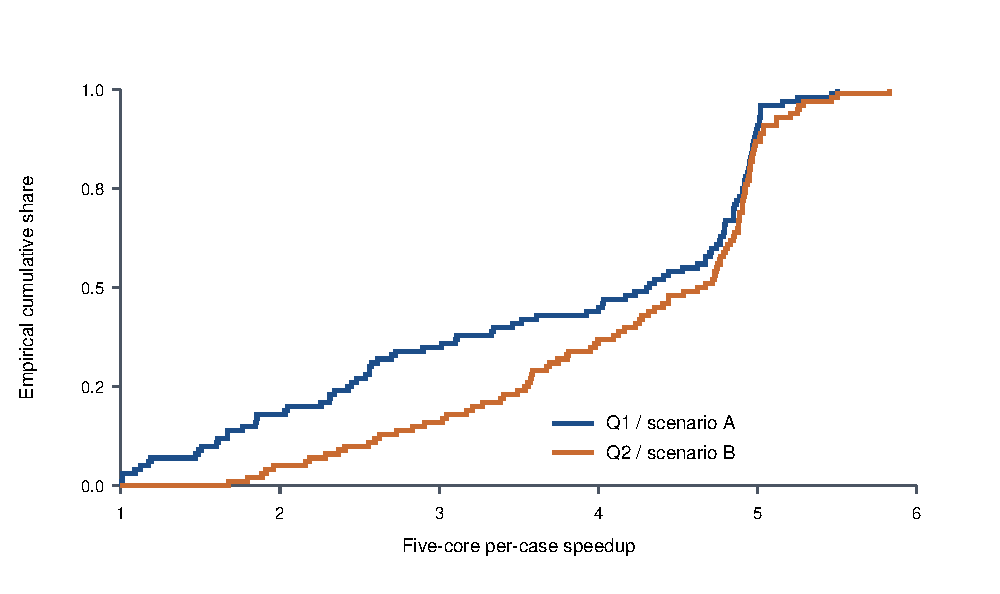
\includegraphics[width=0.82\linewidth,height=0.52\textheight,keepaspectratio]{../图表/paper_diagnostics/five_core_speedup_cdf.pdf}
\caption{问题一、二五核逐图加速比的经验累积分布；数据来自冻结的各 100 条五核记录}\label{fig:fivecore-cdf}
\end{figure}

\subsection{大图周期贡献与等权指标的资源分配冲突}
问题二五核总周期为 $65\,769\,876$。按五核绝对周期从高到低排序，前十张图的周期合计约占总周期的 $70.6449\%$。这十张图是第 $67,28,79,72,14,73,97,16,91,21$ 图；其中第 $67$ 图五核仍需 $13\,461\,153$ 周期，单独贡献超过总周期的五分之一。这样的集中度说明若目标是减少这一批图的\emph{总运行负担}，改善少数大图的绝对周期很重要。但赛题主图的 $\overline S_5$ 每张图只占 $1/100$，大图改进对规定平均加速比未必同样显著。两种目标之间没有逻辑矛盾，区别在于“每个 case 公平等权”和“每个 cycle 公平等权”的利益分配。

可用边际效应精确表示这层差异。若只把第 $i$ 图五核时间从 $T_i$ 降至 $T_i-\delta$，其中 $0<\delta<T_i$，则平均加速比提升
\begin{equation}\label{eq:mean-marginal-benefit}
\Delta\overline S_5=
\frac{T_{i,1}^{0}}{100}
\left(\frac{1}{T_i-\delta}-\frac{1}{T_i}\right)
=\frac{T_{i,1}^{0}\,\delta}{100T_i(T_i-\delta)},
\end{equation}
而总周期直接减少 $\delta$。对于小改动 $\delta\ll T_i$，均值的边际系数约为 $T_{i,1}^{0}/(100T_i^2)$；总周期的边际系数恒为 $1$。由此，若把全部 CPU 搜索时间都给绝对周期最大的图，可能提升总周期比却错过对平均加速比更有效的小图；反过来，只追逐易于抬高逐图比例的小图，又可能让最耗时图占据绝大部分总周期。本文先完成全一百图的合法交付，再依据两种指标分别分析，不用一种统计量替代另一种。

在求解预算上，可以考虑一个受限的优先级分配模型。设每张图的额外评价机会为 $b_i$，主机总预算为 $B_{\rm CPU}$，官方评估一次的预计成本为 $c_i$，则形式上约束 $\sum_i b_ic_i\le B_{\rm CPU}$。若仅以总周期为目标，可估计每次机会的预计绝对改进 $\widehat g_i^{\rm cycles}$；若以题目平均加速比为目标，可估计式\eqref{eq:mean-marginal-benefit}对应的 $\widehat g_i^{\rm mean}$。两类收益都有代理误差，不应通过自适应地不断尝试直到某图变好来制造不公平预算。交付版采用固定每配置上限和结构门控，保证可复核；上述模型是解释下一轮如何在\emph{额外、独立的开发预算}里决定优先分析哪类图，而非宣称当前百图成绩已通过跨图最优预算分配取得。

\subsection{L2 收益分布与负收益口径}
问题三的五核同核时间比 $g_i=T^B_{i,5}/T^{L2}_{i,5}$ 分布也不均匀。其最小值和前四分之一分位数均为 $1$，中位数约 $1.004997$，四分之三位约 $1.031714$，九十分位约 $1.060672$，最大值约 $1.176398$。图\ref{fig:l2-ratio-hist}显示 $29$ 张图的五核时间完全持平、$25$ 张图在 $1$ 到 $1.01$ 之间，只有 $8$ 张图的时间比达到或超过 $1.08$。因此 $1.022567$ 的五核逐图平均同核比主要来自具有明确缓存机会的那部分图，不能把它解释为所有算例都取得约 $2.26\%$ 的均匀改进。
\begin{figure}[!htbp]\centering
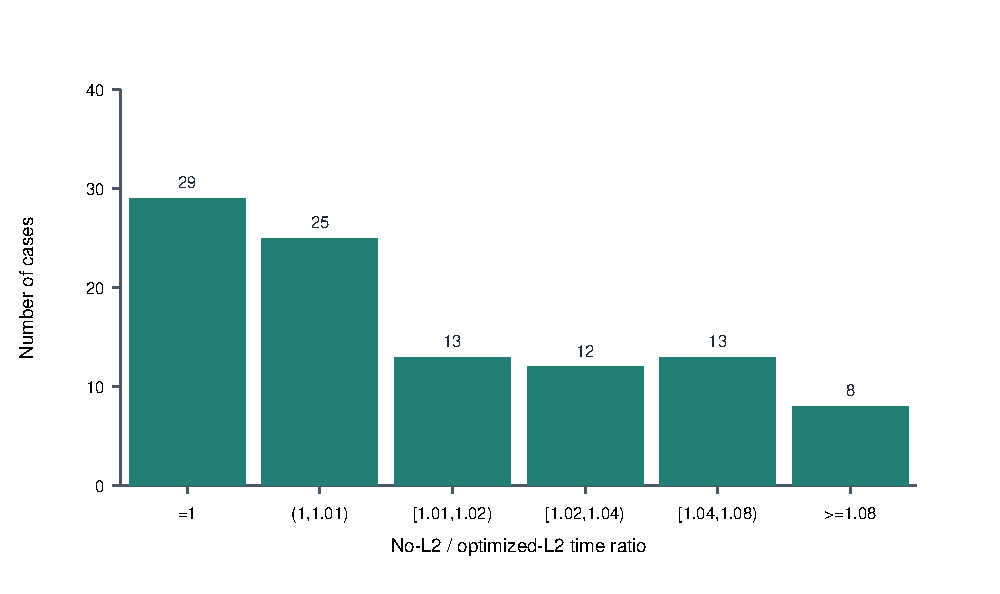
\includegraphics[width=0.82\linewidth,height=0.52\textheight,keepaspectratio]{../图表/paper_diagnostics/five_core_l2_ratio.pdf}
\caption{问题三五核同图同核无 L2 与优化 L2 的时间比直方图}\label{fig:l2-ratio-hist}
\end{figure}

五核直方图恰好没有相对无 L2 的退步，不能据此隐去其它核数下的四组负例。对一百图中每张图的 $k$ 核分别优化后，跨场景比值的符号会随 $k$ 改变：同一图在一核或五核可能命中有效，在两核却因 FIFO 顺序、DDR 与同步路径耦合略慢。图\ref{fig:l2-ratio-hist}只展示 $k=5$ 的横截面；表\ref{tab:q3-total-cycle}和附录五百行保留全部 $k=1,\ldots,5$。若把仅五核的无负例错写成全五百组无负例，就会和第 $67$ 图双核等正式结果冲突。由此也可见，报告分布时必须明确图集合、核数、场景和方案是否固定，否则一个“平均收益”没有可验证的分母。

\subsection{结果图生成的最小复现合同}
新增的两张分布图由仓库\texttt{图表/论文诊断图.py}从冻结的三份 CSV 重新生成，不读取开发阶段的搜索日志。程序先筛选 \texttt{cores=5} 并断言每组恰有 $100$ 行，再按实测 \texttt{speedup} 或 \texttt{combined\_ratio} 绘图；直方图还检查六个桶的数量总和为 $100$。这一检查只保障绘图输入的基本形状，不能代替上述方案层和官方评价层核验。图中的英文坐标是为了避免图形库字体差异影响跨平台复现，中文标题与物理解释在图注和正文给出。若后来修改了逐例方案，应重新生成 CSV 与图表并更新交付版本，而不能让正文数值、图像与附录指向不同的运行。
